\documentclass[tikz,border=3mm]{standalone}
\usepackage{tikz}
\usetikzlibrary{angles,quotes,calc,intersections}
\begin{document}
% TikZ 1

\begin{tikzpicture}[scale=1]
\node[draw,thick,rounded corners=1mm] (E) at (0,0) {Entrada};
\node[draw,thick,rounded corners=1mm] (P1) at (3,0) {Passo 1};
\node[draw,thick,rounded corners=1mm] (P2) at (6,0) {Passo 2};
\node[draw,thick,rounded corners=1mm] (S) at (9,0) {Saida};
\draw[->,thick] (E)--(P1);
\draw[->,thick] (P1)--(P2);
\draw[->,thick] (P2)--(S);
\end{tikzpicture}
\hspace{1cm}
% TikZ 2
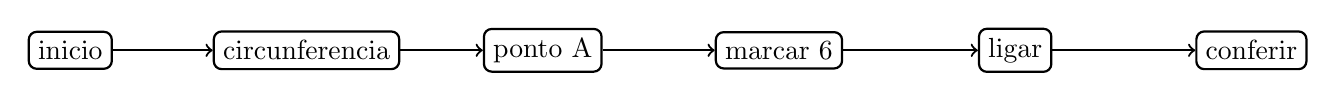
\begin{tikzpicture}[scale=1]
\node[draw,thick,rounded corners=1mm] (I) at (0,0) {inicio};
\node[draw,thick,rounded corners=1mm] (C) at (3,0) {circunferencia};
\node[draw,thick,rounded corners=1mm] (A) at (6,0) {ponto A};
\node[draw,thick,rounded corners=1mm] (M) at (9,0) {marcar 6};
\node[draw,thick,rounded corners=1mm] (L) at (12,0) {ligar};
\node[draw,thick,rounded corners=1mm] (F) at (15,0) {conferir};
\draw[->,thick] (I)--(C);
\draw[->,thick] (C)--(A);
\draw[->,thick] (A)--(M);
\draw[->,thick] (M)--(L);
\draw[->,thick] (L)--(F);
\end{tikzpicture}

\vspace{1cm}

% TikZ 3
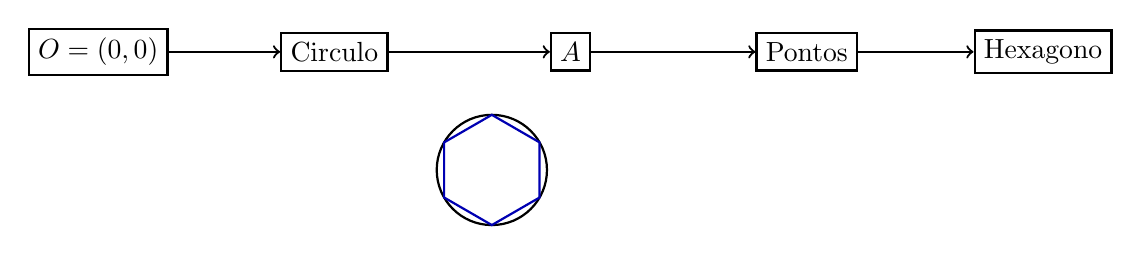
\begin{tikzpicture}[scale=1]
\node[draw,thick] (O) at (0,1.5) {$O=(0,0)$};
\node[draw,thick] (C) at (3,1.5) {Circulo};
\node[draw,thick] (A) at (6,1.5) {$A$};
\node[draw,thick] (P) at (9,1.5) {Pontos};
\node[draw,thick] (H) at (12,1.5) {Hexagono};
\draw[->,thick] (O)--(C);
\draw[->,thick] (C)--(A);
\draw[->,thick] (A)--(P);
\draw[->,thick] (P)--(H);
\draw[thick] (5,0) circle (.7);
\draw[thick,blue!70!black] (5,.7)--(5.606,.35)--(5.606,-.35)--(5,-.7)--(4.394,-.35)--(4.394,.35)--cycle;
\end{tikzpicture}
\end{document}
